% Drawing 142/06-10 -- folder 142, batch 06, archive page 109 (PDF page 110).
% Transcription: Sphère inférieure : pôles marqués $-\zeta$ et $-\bar\zeta$ (lecture incertaine), cercles autour de $\infty$ (point $R^+_\infty$), de $0$ (point $R_0$) et de $1$ ; chemins $c^\pm_1$, $d^\pm_1$, $b^\pm_1$, $a^{\pm\pm}_1$, $s^\pm_1$, le point $Q_1$. À côté : « \uncertain{stable} par \uncertain{symétrie} \uncertain{autour} de l'axe ».
% Kind: sphere with small circles and paths. Method 2 (schematic redraw from the facsimile). Status: partial.
% Notes: Upside-down half of p. 109, redrawn upright. Pencil outline and equator; the poles (labels read like -zeta with a bar at the top and -zeta at the bottom, uncertain as in the transcription); the inked circle round infinity with R_infty^+, the circle round 0 with R_0, the pencil circle round 1 with s_1^+-, a_1^{+-+-}; Q_1 near -1; the thick arrow b_1^- from Q_1 to R_infty^+, dashed paths c_1^+-, d_1^+- to the poles. The note "stable par symetrie autour de l'axe" on the right is left as text (its reading is uncertain).
% Coordinates: 1 unit = 1 mm = 1/100 of the crop width (bbox in page fractions: [0.156, 0.28, 0.548, 0.45]).
% Redrawn by Claude (claude-opus-5-5), issue #73, 2026-11-07; not checked by a human; not compiled (no TeX in the session).
% Rights: reproduces part of the work -- behind RENDER_TRANSCRIPTS, never published by itself.
\documentclass[tikz,border=3pt]{standalone}
\usepackage{amsmath,amssymb}
\usetikzlibrary{patterns,arrows.meta}
\tikzset{pencil/.style={black!45}, struck/.style={black!35}, mark/.style={circle,draw,inner sep=1.3pt}, pt/.style={circle,fill,inner sep=0.9pt}, opt/.style={circle,draw,fill=white,inner sep=1.1pt}}
\begin{document}
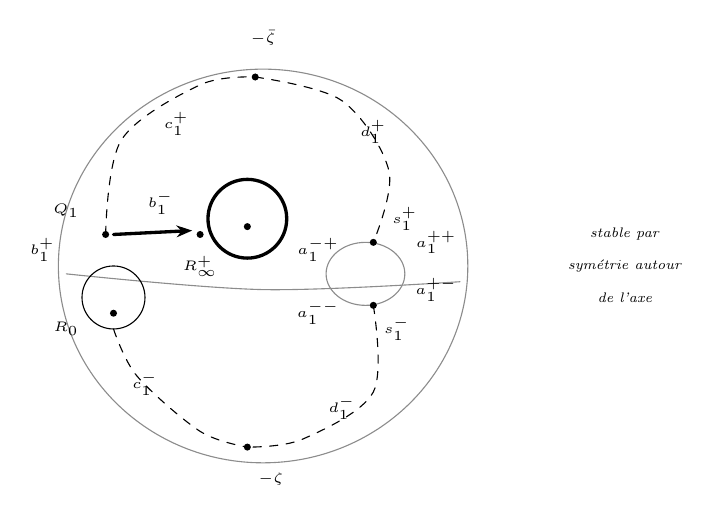
\begin{tikzpicture}[x=1mm,y=1mm,line cap=round,line join=round,font=\scriptsize]
\draw[pencil] (30,-34) ellipse[x radius=26, y radius=25];
\node[pt] at (29,-10) {};
\node[pt] at (28,-57) {};
\node[pt] at (10,-30) {};
\draw[pencil] plot[smooth, tension=0.55] coordinates {(5,-35) (30,-37) (55,-36)};
\draw[very thick] (28,-28) circle[radius=5];
\node[pt] at (28,-29) {};
\node[pt] at (22,-30) {};
\draw[-{Stealth[length=2mm]},very thick] (11,-30) -- (21,-29.5);
\draw (11,-38) circle[radius=4];
\node[pt] at (11,-40) {};
\draw[pencil] (43,-35) ellipse[x radius=5, y radius=4];
\node[pt] at (44,-31) {};
\node[pt] at (44,-39) {};
\draw[dashed] plot[smooth, tension=0.55] coordinates {(10,-30) (12,-18) (22,-11) (29,-10)};
\draw[dashed] plot[smooth, tension=0.55] coordinates {(11,-42) (14,-48) (22,-55) (28,-57)};
\draw[dashed] plot[smooth, tension=0.55] coordinates {(29,-10) (40,-13) (46,-22) (44,-31)};
\draw[dashed] plot[smooth, tension=0.55] coordinates {(44,-39) (44,-50) (35,-56) (28,-57)};
\node[inner sep=1pt] at (30,-5) {\tiny $-\bar\zeta$};
\node[inner sep=1pt] at (31,-61) {\tiny $-\zeta$};
\node[inner sep=1pt] at (5,-27) {\tiny $Q_1$};
\node[inner sep=1pt] at (2,-32) {\tiny $b_1^{+}$};
\node[inner sep=1pt] at (17,-26) {\tiny $b_1^{-}$};
\node[inner sep=1pt] at (22,-34) {\tiny $R_\infty^{+}$};
\node[inner sep=1pt] at (5,-42) {\tiny $R_0$};
\node[inner sep=1pt] at (19,-16) {\tiny $c_1^{+}$};
\node[inner sep=1pt] at (15,-49) {\tiny $c_1^{-}$};
\node[inner sep=1pt] at (44,-17) {\tiny $d_1^{+}$};
\node[inner sep=1pt] at (40,-52) {\tiny $d_1^{-}$};
\node[inner sep=1pt] at (48,-28) {\tiny $s_1^{+}$};
\node[inner sep=1pt] at (47,-42) {\tiny $s_1^{-}$};
\node[inner sep=1pt] at (37,-32) {\tiny $a_1^{-+}$};
\node[inner sep=1pt] at (52,-31) {\tiny $a_1^{++}$};
\node[inner sep=1pt] at (52,-37) {\tiny $a_1^{+-}$};
\node[inner sep=1pt] at (37,-40) {\tiny $a_1^{--}$};
\node[inner sep=1pt] at (76,-30) {\tiny \textit{stable par}};
\node[inner sep=1pt] at (76,-34) {\tiny \textit{sym\'etrie autour}};
\node[inner sep=1pt] at (76,-38) {\tiny \textit{de l'axe}};
\end{tikzpicture}
\end{document}
